% STATUS: ACTIVE -- Kalman filter and observability matrix, built up one part at a time (first-order gain model).
% ======================================================
% Compile: xelatex 0927_kf_obs_stepwise.tex   (from reference/eq17_analysis/derivation/)
% Notation: 0921_5state_noap_simple.tex (teacher chain) with delta a removed; Kalman filter = Meng dissertation (4.12)-(4.15),
%           lambda_f = 1, gain L with entries ell_ij (teacher's closed-loop estimator).
% Parts: 1 observability matrix | 2 why 1/P (information) | 3 Kalman filter prediction and update, entry by entry |
%        4 the link | 5 the truth moves: weighted average, a'_x and speed.
% Part 5 figures: fig_noap_weighted_average_check.png (plot_5state_noap_weighted_average_check.m),
%                 fig_noap_weight_per_height.png (plot_5state_noap_weight_per_height.m); runs ladder_ramp16_Td{5,15}_lf1_o1.mat
% Equations only (derivation-workflow rule 10).
% ======================================================
\documentclass[11pt,a4paper]{ctexart}
\usepackage[fleqn]{amsmath}
\usepackage{amssymb,bm}
\usepackage{graphicx}
\graphicspath{{figures/}}
\setlength{\mathindent}{0pt}
\usepackage{geometry}
\geometry{margin=2.0cm}
\setlength{\parindent}{0pt}
\setlength{\parskip}{0.3em}
\setlength{\abovedisplayskip}{4pt}
\setlength{\belowdisplayskip}{4pt}
\newcommand{\lc}{\lambda_c}
\newcommand{\hd}[1]{\par\medskip\noindent\underline{\textbf{#1}}\par\nobreak\vspace{0.2ex}}
\pagestyle{plain}

\begin{document}

\begin{center}\textbf{\large Kalman filter and observability matrix, step by step (first-order gain model)}\end{center}

%======================================================================
\section*{Model}

\[
\begin{aligned}
\delta x_1[k+1] &= \delta x_2[k] \\
\delta x_2[k+1] &= \delta x_3[k] \\
\delta x_3[k+1] &= \lc \cdot \delta x_3[k] - F_{dx}[k]\cdot e_{a_x}[k] - \varepsilon[k] \\
a_x[k+1] &= a_x[k]
\end{aligned}
\qquad\qquad
\begin{aligned}
y_1[k] &= \delta x_m[k] = \delta x_1[k] + n_x[k] \\
y_2[k] &= a_{xm}[k] = a_x[k] + n_a[k]
\end{aligned}
\]
\[
\mathbf{e} = \begin{bmatrix} e_{\delta x_1} \\ e_{\delta x_2} \\ e_{\delta x_3} \\ e_{a_x} \end{bmatrix}, \quad
\mathbf{F}_e[k] =
\begin{bmatrix}
0 & 1 & 0 & 0 \\
0 & 0 & 1 & 0 \\
0 & 0 & \lc & -F_{dx}[k] \\
0 & 0 & 0 & 1
\end{bmatrix}, \quad
\mathbf{H} = \begin{bmatrix} \mathbf{H}_1 \\ \mathbf{H}_2 \end{bmatrix} =
\begin{bmatrix}
1 & 0 & 0 & 0 \\
0 & 0 & 0 & 1
\end{bmatrix}
\]
\[
\mathbf{Q} = \mathrm{diag}(0, 0, Q_{33}, 0), \quad
\mathbf{R} = \mathrm{diag}(R_1, R_2), \qquad
Q_{33} = \mathrm{Var}(\varepsilon), \quad R_1 = \mathrm{Var}(n_x), \quad R_2 = \mathrm{Var}(n_a)
\]
\[
F_{dx} = \big(1 + (1-\lc)d\big)\,\frac{\Delta x_d}{\hat a_x} \qquad (\text{constant velocity})
\]

%======================================================================
\section{Part 1: observability matrix}

\hd{1.1 What the sensors show: measurement minus its prediction}
\[
\begin{aligned}
e_{y_1}[k] &= y_1[k] - \delta\hat x_1[k] = \big(\delta x_1[k] - \delta\hat x_1[k]\big) + n_x[k] = e_{\delta x_1}[k] + n_x[k] \\
e_{y_2}[k] &= y_2[k] - \hat a_x[k] \;\;\,= \big(a_x[k] - \hat a_x[k]\big) + n_a[k] \;\;\,= e_{a_x}[k] + n_a[k]
\end{aligned}
\]

\hd{1.2 How an estimation error moves from one step to the next (no update, no noise)}
\[
\begin{aligned}
e_{\delta x_1}[k+1] &= e_{\delta x_2}[k] \\
e_{\delta x_2}[k+1] &= e_{\delta x_3}[k] \\
e_{\delta x_3}[k+1] &= \lc \cdot e_{\delta x_3}[k] - F_{dx}[k]\cdot e_{a_x}[k] \\
e_{a_x}[k+1] &= e_{a_x}[k]
\end{aligned}
\]

\hd{1.3 $e_{y_1}$ at step $k_0+j$, written with the errors at step $k_0$ (1.1 then 1.2 applied $j$ times)}
\[
\begin{aligned}
e_{y_1}[k_0] &= e_{\delta x_1}[k_0] \\
&= 1\cdot e_{\delta x_1}[k_0] + 0\cdot e_{\delta x_2}[k_0] + 0\cdot e_{\delta x_3}[k_0] + 0\cdot e_{a_x}[k_0] \\[1ex]
e_{y_1}[k_0+1] &= e_{\delta x_1}[k_0+1] = e_{\delta x_2}[k_0] \\
&= 0\cdot e_{\delta x_1}[k_0] + 1\cdot e_{\delta x_2}[k_0] + 0\cdot e_{\delta x_3}[k_0] + 0\cdot e_{a_x}[k_0] \\[1ex]
e_{y_1}[k_0+2] &= e_{\delta x_1}[k_0+2] = e_{\delta x_2}[k_0+1] = e_{\delta x_3}[k_0] \\
&= 0\cdot e_{\delta x_1}[k_0] + 0\cdot e_{\delta x_2}[k_0] + 1\cdot e_{\delta x_3}[k_0] + 0\cdot e_{a_x}[k_0] \\[1ex]
e_{y_1}[k_0+3] &= e_{\delta x_3}[k_0+1] = \lc\, e_{\delta x_3}[k_0] - F_{dx}[k_0]\, e_{a_x}[k_0] \\
&= 0\cdot e_{\delta x_1}[k_0] + 0\cdot e_{\delta x_2}[k_0] + \lc\cdot e_{\delta x_3}[k_0] - F_{dx}[k_0]\cdot e_{a_x}[k_0] \\[1ex]
e_{y_1}[k_0+4] &= e_{\delta x_3}[k_0+2] = \lc\, e_{\delta x_3}[k_0+1] - F_{dx}[k_0+1]\, e_{a_x}[k_0+1] \\
&= \lc\big(\lc\, e_{\delta x_3}[k_0] - F_{dx}[k_0]\, e_{a_x}[k_0]\big) - F_{dx}[k_0+1]\, e_{a_x}[k_0] \\
&= 0\cdot e_{\delta x_1}[k_0] + 0\cdot e_{\delta x_2}[k_0] + \lc^2\cdot e_{\delta x_3}[k_0] - \big(\lc F_{dx}[k_0] + F_{dx}[k_0+1]\big)\cdot e_{a_x}[k_0] \\[1ex]
e_{y_1}[k_0+j] &= 0\cdot e_{\delta x_1}[k_0] + 0\cdot e_{\delta x_2}[k_0] + \lc^{\,j-2}\cdot e_{\delta x_3}[k_0]
- \Big(\textstyle\sum_{i=0}^{j-3}\lc^{\,j-3-i}F_{dx}[k_0+i]\Big)\cdot e_{a_x}[k_0], \qquad j \ge 3
\end{aligned}
\]

\hd{1.4 $e_{y_2}$ at step $k_0+j$}
\[
e_{y_2}[k_0+j] = e_{a_x}[k_0+j] = e_{a_x}[k_0]
= 0\cdot e_{\delta x_1}[k_0] + 0\cdot e_{\delta x_2}[k_0] + 0\cdot e_{\delta x_3}[k_0] + 1\cdot e_{a_x}[k_0]
\]

\hd{1.5 The coefficients, collected: observability matrix $\mathbf{O}$}
\[
\begin{bmatrix} e_{y_1}[k_0] \\ e_{y_2}[k_0] \\ e_{y_1}[k_0+1] \\ e_{y_2}[k_0+1] \\ e_{y_1}[k_0+2] \\ e_{y_2}[k_0+2] \\ e_{y_1}[k_0+3] \\ e_{y_2}[k_0+3] \\ e_{y_1}[k_0+4] \\ \vdots \end{bmatrix}
=
\underbrace{\begin{bmatrix}
1 & 0 & 0 & 0 \\
0 & 0 & 0 & 1 \\
0 & 1 & 0 & 0 \\
0 & 0 & 0 & 1 \\
0 & 0 & 1 & 0 \\
0 & 0 & 0 & 1 \\
0 & 0 & \lc & -F_{dx}[k_0] \\
0 & 0 & 0 & 1 \\
0 & 0 & \lc^2 & -\lc F_{dx}[k_0] - F_{dx}[k_0+1] \\
\vdots & \vdots & \vdots & \vdots
\end{bmatrix}}_{\mathbf{O}}
\begin{bmatrix} e_{\delta x_1}[k_0] \\ e_{\delta x_2}[k_0] \\ e_{\delta x_3}[k_0] \\ e_{a_x}[k_0] \end{bmatrix}
+ \text{noise}
\]
\[
\text{row } j \text{ of } \mathbf{O} = \mathbf{H}\,\bm{\Phi}(k_0+j,k_0), \qquad
\bm{\Phi}(k_0+j,k_0) = \mathbf{F}_e[k_0+j-1]\cdots\mathbf{F}_e[k_0]
\]

\hd{1.6 The $e_{a_x}$ column alone ($F_{dx}$ constant)}
\[
\begin{aligned}
e_{y_2}[k_0+j] &= 1\cdot e_{a_x}[k_0] + n_a \qquad (j \ge 0) \\
e_{y_1}[k_0+j] &= c_{1,j}\cdot e_{a_x}[k_0] + (\text{position errors}) + n_x \qquad (j \ge 3) \\
c_{1,j} &= -F_{dx}\big(1 + \lc + \cdots + \lc^{\,j-3}\big) \;\to\; -\frac{F_{dx}}{1-\lc}
\end{aligned}
\]

%======================================================================
\section{Part 2: information on $a_x$}

\hd{2.1 One unknown $e$, one reading $z = c\,e + n$, $\mathrm{Var}(n) = R$, prior variance $P$}
\[
\begin{aligned}
J(e) &= \frac{e^2}{P} + \frac{(z - c\,e)^2}{R} \\
\frac{dJ}{de} &= \frac{2e}{P} - \frac{2c\,(z - c\,e)}{R} = 0
\;\Rightarrow\; \hat e = \frac{c\,z/R}{1/P + c^2/R} \\
\frac{1}{P_{\text{new}}} &= \frac{1}{2}\frac{d^2J}{de^2} = \frac{1}{P} + \frac{c^2}{R}
\end{aligned}
\]

\hd{2.2 $y_2$ readings of $e_{a_x}$ ($c = 1$)}
\[
\frac{1}{P_{aa}[k]} = \frac{1}{P_{aa}[k-1]} + \frac{1^2}{R_2}
\;\Rightarrow\; \frac{1}{P_{aa}[k_0+N]} = \frac{1}{P_{aa}[k_0]} + \frac{N}{R_2}
\]

\hd{2.3 $y_1$ readings of $e_{a_x}$ ($c = c_{1,j}$, position errors known)}
\[
\frac{1}{P_{aa}[k_0+N]} = \frac{1}{P_{aa}[k_0]} + \sum_{j=3}^{N-1}\frac{c_{1,j}^2}{R_1}
\]

\hd{2.4 Both, and all four errors at once}
\[
\begin{aligned}
\frac{1}{P_{aa}[k_0+N]} &\le \frac{1}{P_{aa}[k_0]} + \frac{N}{R_2} + \sum_{j=3}^{N-1}\frac{c_{1,j}^2}{R_1} \qquad (\text{equality when the position errors are known}) \\
\mathbf{P}^{-1}[k_0 \,|\, k_0+N-1] &= \mathbf{P}^{-1}[k_0] + \mathbf{O}^{\top}\mathbf{R}^{-1}\mathbf{O}, \qquad
\big(\mathbf{O}^{\top}\mathbf{R}^{-1}\mathbf{O}\big)_{aa} = \frac{N}{R_2} + \sum_{j}\frac{c_{1,j}^2}{R_1} \qquad (\mathbf{Q} = 0)
\end{aligned}
\]

%======================================================================
\section{Part 3: Kalman filter, entry by entry}

\hd{3.1 Prediction of the state}
\[
\delta\hat x_1^f[k] = \delta\hat x_2[k-1], \quad
\delta\hat x_2^f[k] = \delta\hat x_3[k-1], \quad
\delta\hat x_3^f[k] = \lc\,\delta\hat x_3[k-1], \quad
\hat a_x^f[k] = \hat a_x[k-1]
\]

\hd{3.2 Prediction of $\mathbf{P}$}
\[
\begin{aligned}
\mathbf{P}^f &= \mathbf{F}_e\,\mathbf{P}\,\mathbf{F}_e^{\top} + \mathbf{Q}, \qquad
\mathbf{r}_1 = [0\;1\;0\;0],\;\; \mathbf{r}_2 = [0\;0\;1\;0],\;\; \mathbf{r}_3 = [0\;0\;\lc\;{-F_{dx}}],\;\; \mathbf{r}_4 = [0\;0\;0\;1] \\
P^f_{ij} &= \mathbf{r}_i\,\mathbf{P}\,\mathbf{r}_j^{\top} + Q_{ij}
\end{aligned}
\]
\[
\begin{aligned}
P^f_{11} &= P_{22} & P^f_{12} &= P_{23} & P^f_{13} &= \lc P_{23} - F_{dx} P_{2a} & P^f_{1a} &= P_{2a} \\
P^f_{22} &= P_{33} & P^f_{23} &= \lc P_{33} - F_{dx} P_{3a} & P^f_{2a} &= P_{3a} & & \\
P^f_{33} &= \lc^2 P_{33} - 2\lc F_{dx} P_{3a} + F_{dx}^2 P_{aa} + Q_{33} & P^f_{3a} &= \lc P_{3a} - F_{dx} P_{aa} & P^f_{aa} &= P_{aa} & &
\end{aligned}
\]

\hd{3.3 Update with $y_1$ ($\mathbf{H}_1 = [1\;0\;0\;0]$)}
\[
\begin{aligned}
S_1 &= P^f_{11} + R_1, \qquad \ell_{i1} = \frac{P^f_{i1}}{S_1}\;\;(i = 1,2,3,4), \qquad \ell_{41} = \frac{P^f_{a1}}{S_1} \\
\hat{\mathbf{x}}' &= \hat{\mathbf{x}}^f + \mathbf{L}_1\big(y_1 - \delta\hat x_1^f\big) \\
P'_{ij} &= P^f_{ij} - \frac{P^f_{i1}\,P^f_{1j}}{S_1}, \qquad
P'_{aa} = P^f_{aa} - \frac{\big(P^f_{a1}\big)^2}{S_1}
\end{aligned}
\]

\hd{3.4 Update with $y_2$ ($\mathbf{H}_2 = [0\;0\;0\;1]$)}
\[
\begin{aligned}
S_2 &= P'_{aa} + R_2, \qquad \ell_{i2} = \frac{P'_{ia}}{S_2}, \qquad \ell_{42} = \frac{P'_{aa}}{P'_{aa} + R_2} \\
\hat{\mathbf{x}} &= \hat{\mathbf{x}}' + \mathbf{L}_2\big(y_2 - \hat a_x'\big) \\
P_{ij} &= P'_{ij} - \frac{P'_{ia}\,P'_{aj}}{S_2}, \qquad
P_{aa} = P'_{aa} - \frac{\big(P'_{aa}\big)^2}{P'_{aa} + R_2} = \frac{R_2\,P'_{aa}}{P'_{aa} + R_2}
\end{aligned}
\]
\[
(\text{3.3 then 3.4} \;=\; \text{joint update with } \mathbf{H}, \; \mathbf{R} \text{ diagonal})
\]

\hd{3.5 $P_{aa}$ written as $1/P_{aa}$}
\[
\begin{aligned}
\text{3.4:}\quad \frac{1}{P_{aa}} &= \frac{P'_{aa} + R_2}{R_2\,P'_{aa}} = \frac{1}{P'_{aa}} + \frac{1}{R_2} \\
\text{3.3:}\quad \frac{1}{P'_{aa}} &= \frac{1}{P^f_{aa}}\cdot\frac{1}{1 - \dfrac{(P^f_{a1})^2}{P^f_{aa}\,S_1}}
\;\approx\; \frac{1}{P^f_{aa}} + \frac{(P^f_{a1})^2}{(P^f_{aa})^2\,S_1} \\
\text{3.2:}\quad \frac{1}{P^f_{aa}} &= \frac{1}{P_{aa}[k-1]} \\
\frac{1}{P_{aa}[k]} &\approx \frac{1}{P_{aa}[k-1]} + \frac{(P^f_{a1})^2}{(P^f_{aa})^2\,S_1} + \frac{1}{R_2}
\end{aligned}
\]

%======================================================================
\section{Part 4: the link}

\hd{4.1 Prediction only, starting from $P_{1a} = P_{2a} = P_{3a} = 0$, $P_{aa}$ constant}
\[
\begin{aligned}
P_{3a}[k_0+1] &= -F_{dx}[k_0]\,P_{aa} \\
P_{3a}[k_0+2] &= \big(-\lc F_{dx}[k_0] - F_{dx}[k_0+1]\big)\,P_{aa} \\
P_{2a}[k_0+j] &= P_{3a}[k_0+j-1], \qquad P_{1a}[k_0+j] = P_{2a}[k_0+j-1] = P_{3a}[k_0+j-2]
\end{aligned}
\]
\[
\begin{aligned}
P_{ia}[k_0+j] &= \big(\text{coefficient of } e_{a_x}[k_0] \text{ in } e_{\delta x_i}[k_0+j]\text{, 1.3}\big)\cdot P_{aa} \\
P^f_{1a}[k_0+j] &= \big(\text{coefficient of } e_{a_x}[k_0] \text{ in } e_{y_1}[k_0+j]\text{, 1.3}\big)\cdot P_{aa} = c_{1,j}\,P_{aa}
\end{aligned}
\]

\hd{4.2 Put into 3.3 and 3.5}
\[
\ell_{41} = \frac{c_{1,j}\,P_{aa}}{S_1}, \qquad
\frac{(P^f_{a1})^2}{(P^f_{aa})^2\,S_1} = \frac{c_{1,j}^2}{S_1} = \frac{c_{1,j}^2}{P^f_{11} + R_1}, \qquad
\frac{1}{P_{aa}[k]} \approx \frac{1}{P_{aa}[k-1]} + \frac{c_{1,j}^2}{P^f_{11} + R_1} + \frac{1^2}{R_2}
\]
\[
(\text{compare 2.3: } \dfrac{c_{1,j}^2}{R_1} \text{ per } y_1 \text{ row; here } R_1 \to P^f_{11} + R_1)
\]


%======================================================================
\clearpage
\section{Part 5: the truth moves -- average and speed}

\hd{5.1 Weight of each step (Parts 2--4)}
\[
w_j = \frac{1}{P_{aa}[j]} - \frac{1}{P_{aa}[j-1]} \approx \frac{c_{1,j}^2}{P^f_{11}[j] + R_1} + \frac{1}{R_2}, \qquad
W_0 = \frac{1}{P_{aa}[0]}
\]

\hd{5.2 Each step's readings speak about the gain at that step}
\[
\begin{aligned}
y_2[j] &= a_x[j] + n_a[j] \\
J(a_x) &= W_0\big(a_x - \hat a_x[0]\big)^2 + \sum_{j=1}^{k} w_j\big(a_x - a_x[j]\big)^2 \\
\hat a_x[k] &= \frac{W_0\,\hat a_x[0] + \sum_{j=1}^{k} w_j\,a_x[j]}{W_0 + \sum_{j=1}^{k} w_j}
= \kappa_0\,\hat a_x[0] + \sum_{j=1}^{k}\kappa_j\,a_x[j] \\
\kappa_j &= \frac{w_j}{W_0 + \sum_{i=1}^{k} w_i}, \qquad \kappa_0 = \frac{W_0}{W_0 + \sum_{i=1}^{k} w_i}, \qquad \kappa_0 + \sum_{j=1}^{k}\kappa_j = 1
\end{aligned}
\]

\hd{5.3 Estimation error}
\[
e_{a_x}[k] = a_x[k] - \hat a_x[k]
= \kappa_0\big(a_x[k] - \hat a_x[0]\big) + \sum_{j=1}^{k}\kappa_j\,\big(a_x[k] - a_x[j]\big)
\]

\hd{5.4 The change of the truth between step $j$ and step $k$}
\[
a_x[k] - a_x[j] = \sum_{i=j}^{k-1}\big(a_x[i+1] - a_x[i]\big) = \sum_{i=j}^{k-1} a'_x\big(h_d[i]\big)\,\Delta h_d[i],
\qquad a'_x = \frac{d a_x}{d h}
\]
\[
e_{a_x}[k] = \kappa_0\big(a_x[k] - \hat a_x[0]\big) + \sum_{j=1}^{k}\kappa_j \sum_{i=j}^{k-1} a'_x\big(h_d[i]\big)\,\Delta h_d[i]
\]

\hd{5.5 $a'_x$ nearly constant over the weighted steps}
\[
e_{a_x}[k] \approx a'_x\big(h_d[k]\big)\,\Big(h_d[k] - \bar h_{\kappa}[k]\Big), \qquad
\bar h_{\kappa}[k] = \kappa_0\,h_d[0] + \sum_{j=1}^{k}\kappa_j\,h_d[j]
\]

\hd{5.6 Fixed height}
\[
h_d[j] = h_d[k] \;\;\forall j \;\Rightarrow\; a_x[j] = a_x[k] \;\Rightarrow\; e_{a_x}[k] = \kappa_0\big(a_x[k] - \hat a_x[0]\big) \;\xrightarrow{\;k \to \infty\;}\; 0
\]

\hd{5.7 Speed: weight per $R$ travelled (constant velocity, $\Delta h_d = (h_0 - h_b)\,T_s/T_d$)}
\[
\begin{aligned}
y_2:&\quad \frac{1}{R_2}\cdot\frac{T_d}{(h_0 - h_b)\,T_s} \;\propto\; T_d \quad (\text{same at every height}) \\
y_1:&\quad \frac{c_{1}^2}{P^f_{11} + R_1}\cdot\frac{T_d}{(h_0 - h_b)\,T_s}, \quad
c_1 \approx -\frac{1 + (1-\lc)d}{1-\lc}\,\frac{\Delta h_d}{\hat a_x} \;\Rightarrow\; \propto \frac{1}{\hat a_x^2\,T_d} \quad (\text{largest near the wall})
\end{aligned}
\]
\[
\kappa \text{ over } h:\quad y_2 \text{ only} \Rightarrow \text{shape independent of } T_d; \qquad
y_1 \text{ added} \Rightarrow \text{extra weight near the wall} \propto 1/T_d
\]

\clearpage
\section*{Figure for 5.2--5.3: filter vs weighted average with $w_j = \Delta(1/P_{aa})$}
\begin{center}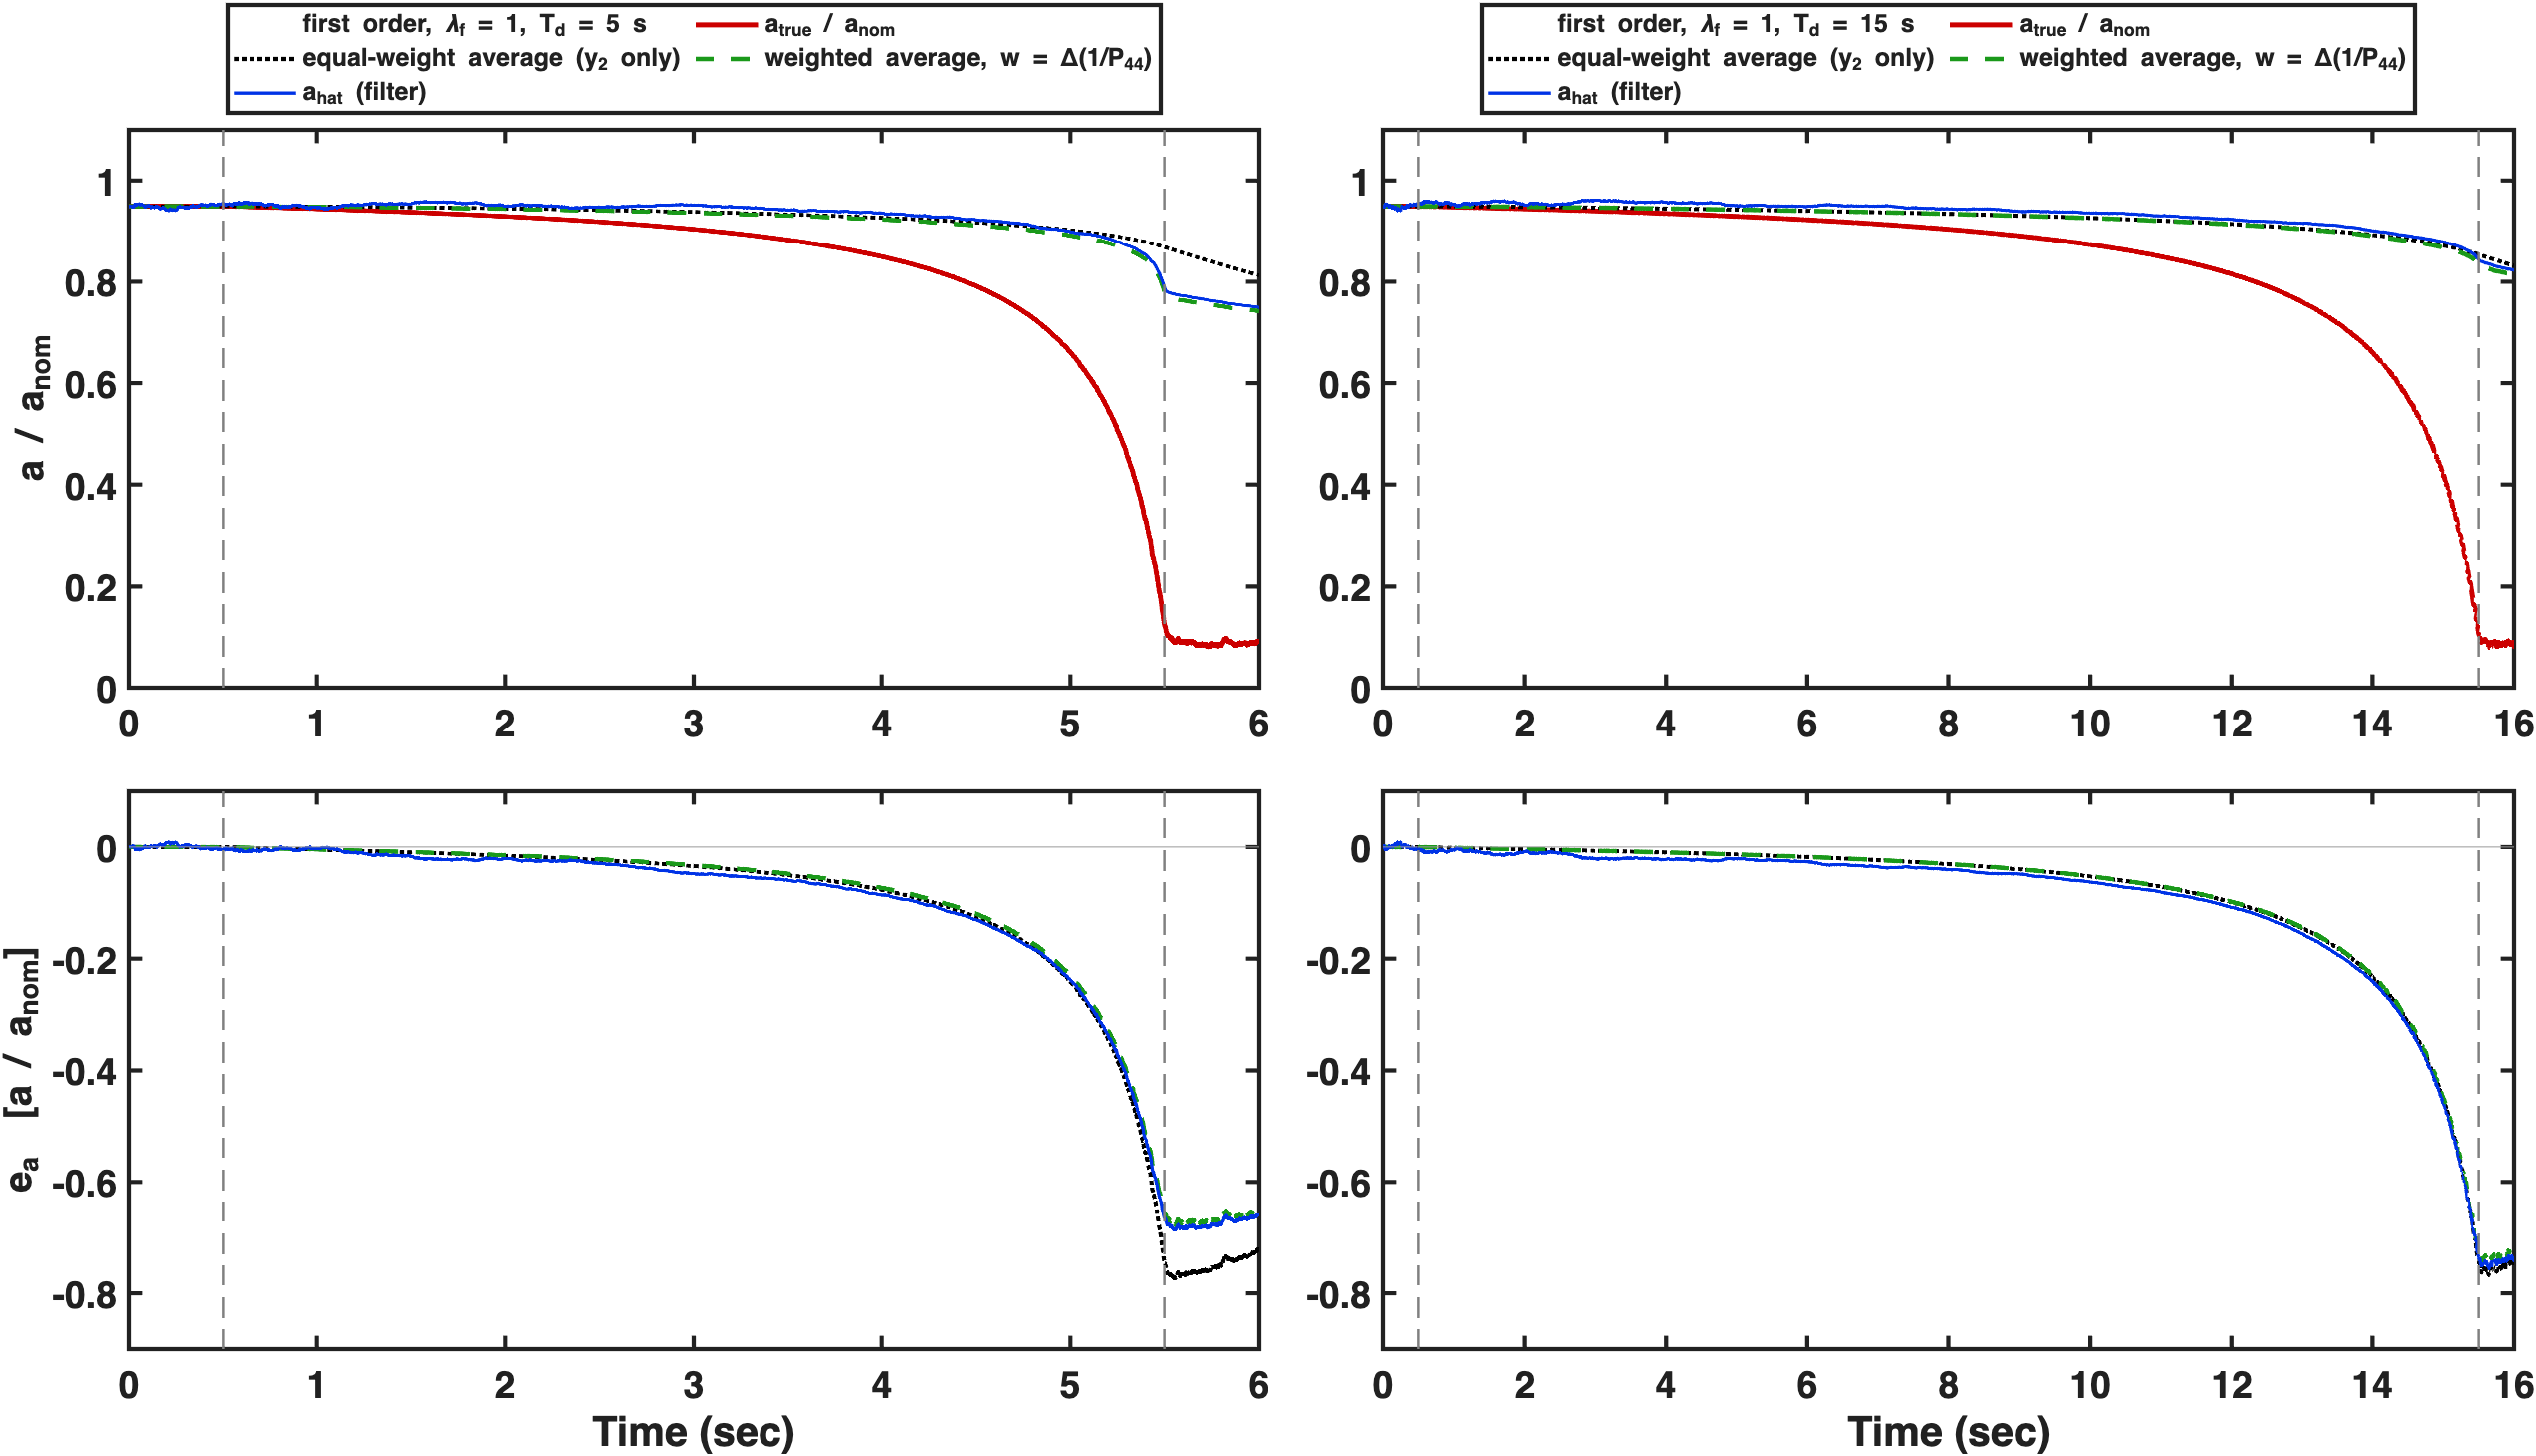
\includegraphics[width=\textwidth]{fig_noap_weighted_average_check.png}\end{center}

\section*{Figure for 5.7: weight added per step and per $R$ travelled}
\begin{center}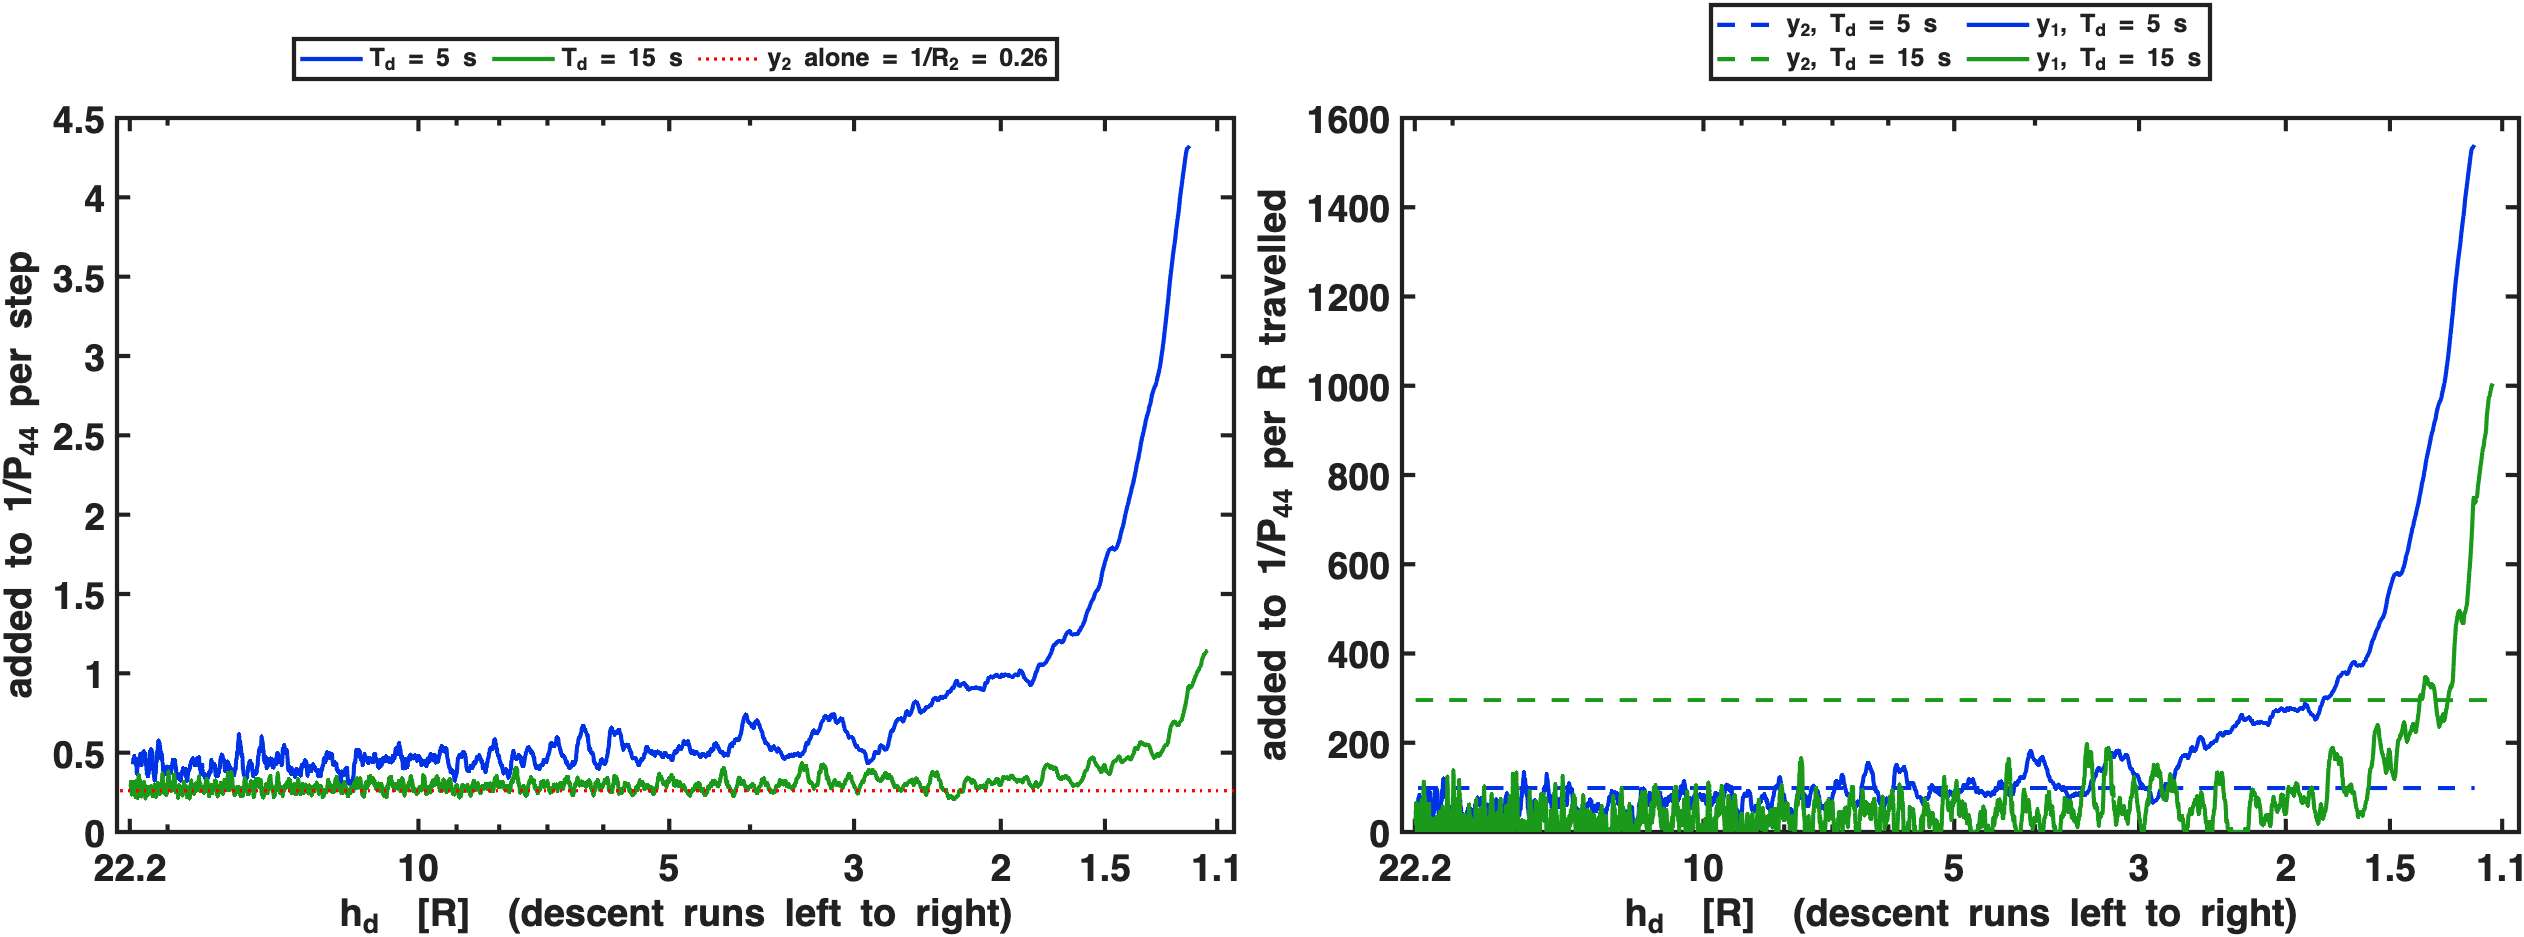
\includegraphics[width=\textwidth]{fig_noap_weight_per_height.png}\end{center}

\end{document}
